Considérons le dessin suivant, où les mesures des angles sont en radians.

\begin{center}
	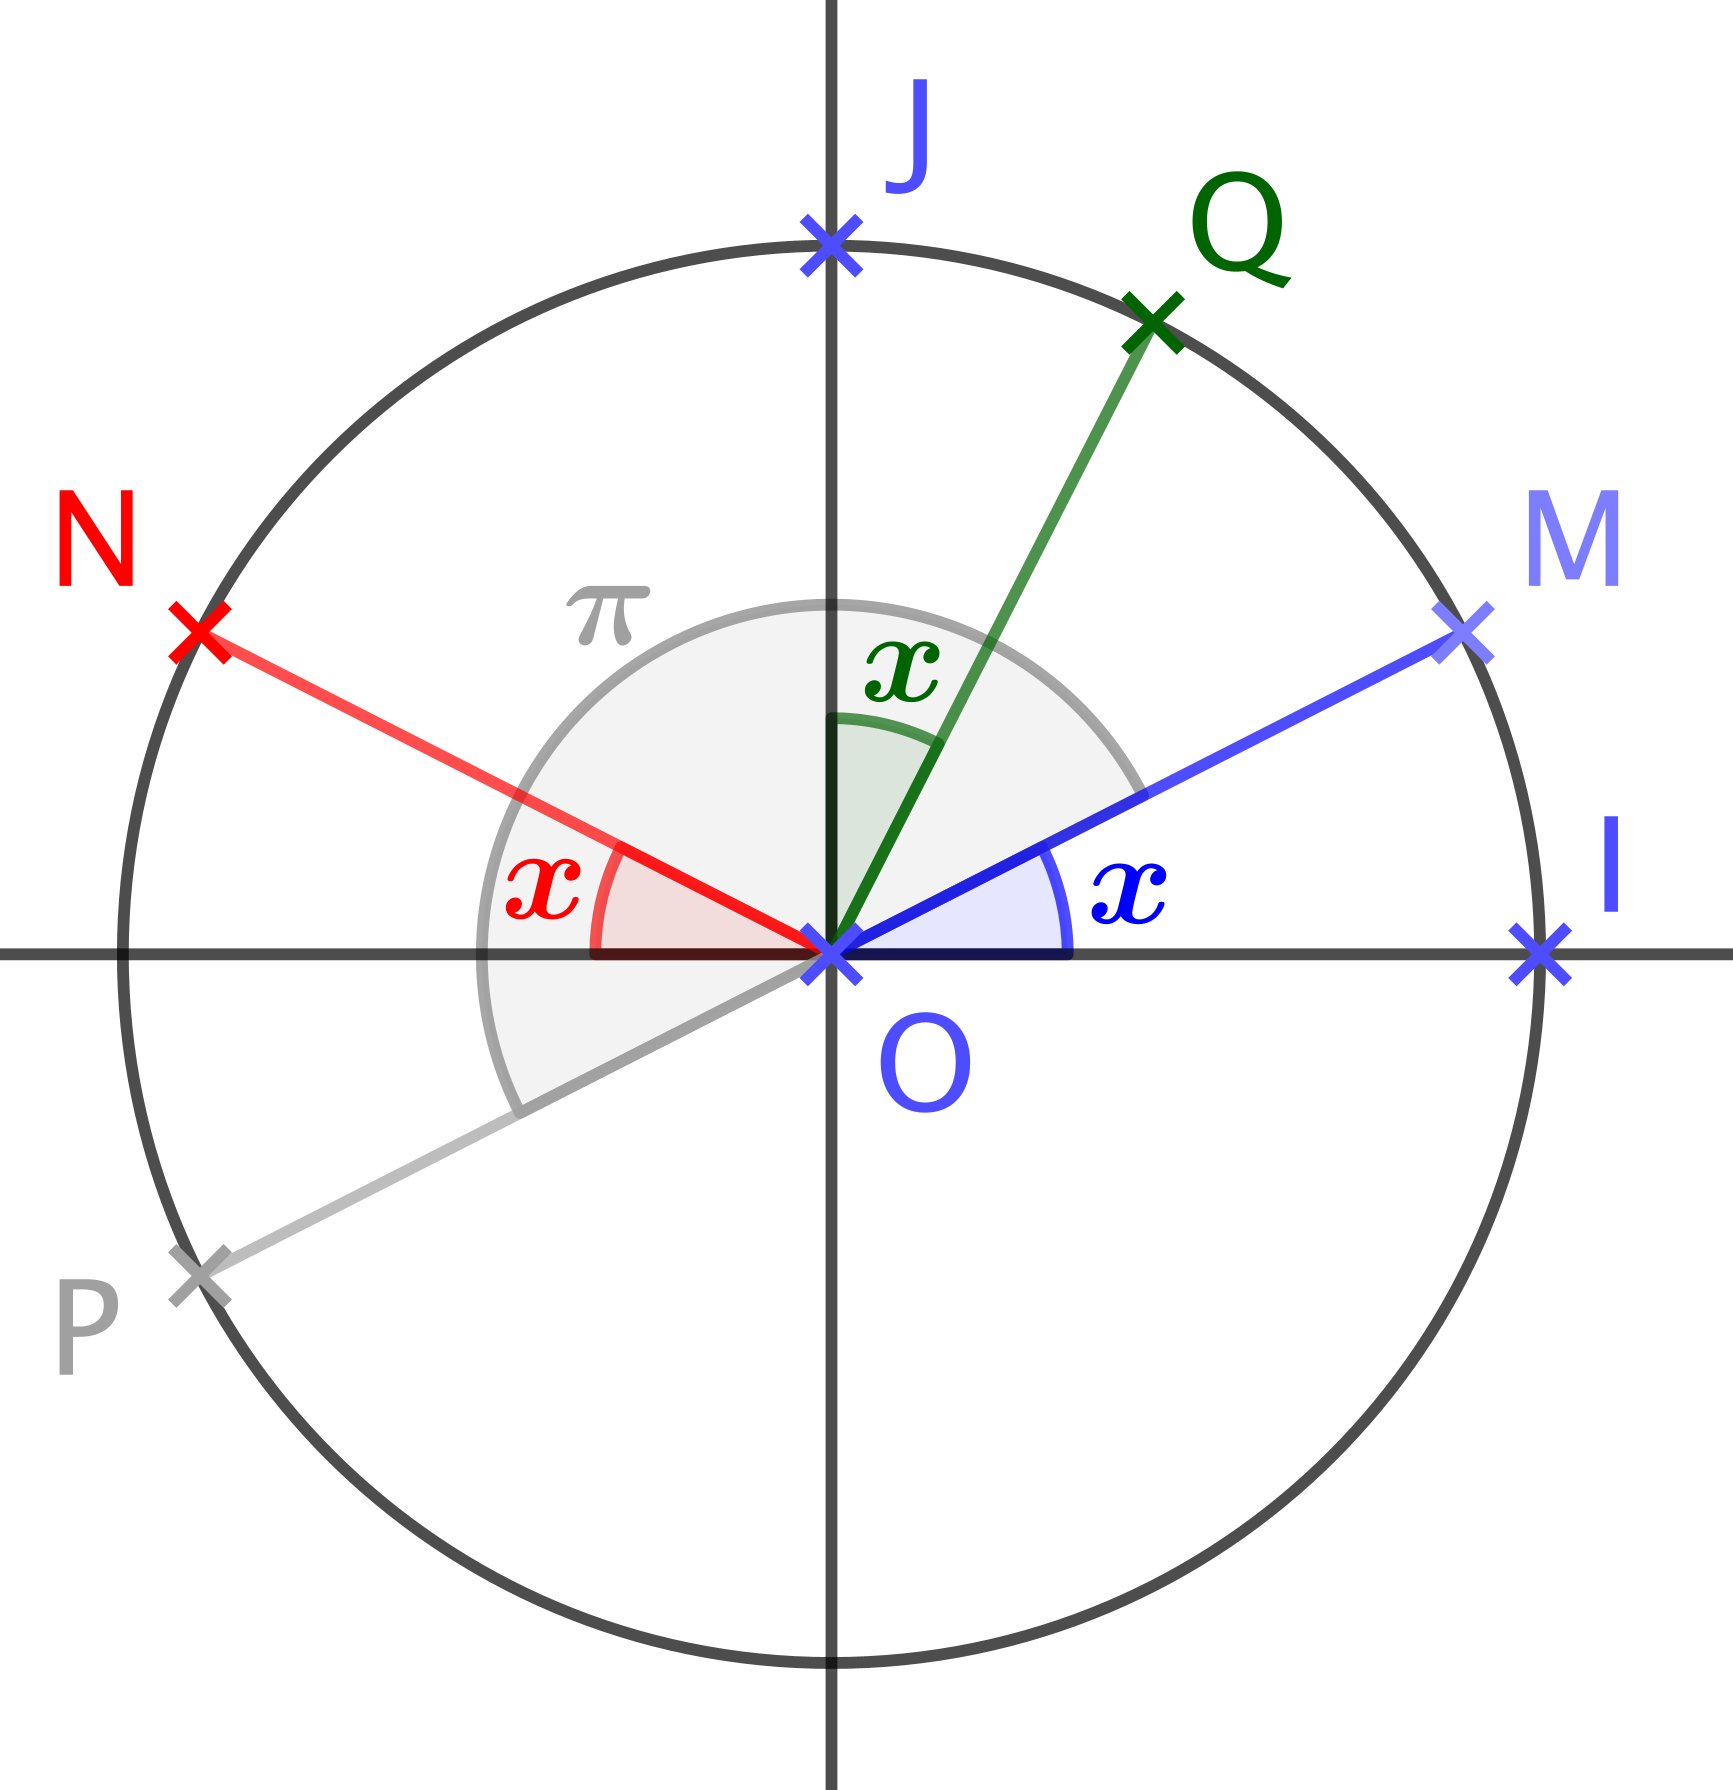
\includegraphics[scale = .7]{one-var-trig-formulas.png}
\end{center}

Via les points $M$, $N$, $P$ et $Q$, il est facile de fournir des arguments géométriques de symétrie justifiant que, sous la condition $x \in \intervalO{0}{\frac{\pi}{4}}$, nous avons:
%
\begin{multicols}{3}
\begin{itemize}[label=\small\textbullet]
	\item $\cos (\pi - x) = - \cos x$

	      \noindent
	      $\sin (\pi - x) = \sin x$ 

	\item $\cos (x + \pi) = - \cos x$

	      \noindent
	      $\sin (x + \pi) = - \sin x$

	\item $\cos \left( \frac{\pi}{2} - x \right) = \sin x$

	      \noindent
	      $\sin \left( \frac{\pi}{2} - x \right) = \cos x$ 
\end{itemize}
\end{multicols}


De nouveau, il serait bien de pouvoir passer, sans plus d'effort, à la validité des formules ci-dessus sur $\RR$ tout entier \emph{(considérer les autres cas n'est pas compliqué, mais c'est pénible)}.
%
Nous allons voir que cela est licite grâce au fait \ref{analytic-identity}, donné plus bas, qui est un peu technique, car il nécessite la notion de fonction analytique.


% ----------- %


\begin{preli} \label{conv-ray}
    Le rayon de convergence $R$ de la série entière complexe $\dsum_{n=0}^{\infty} a_n z^n$ est défini par la formule de Hadamard%
    \footnote{
    	La démonstration va révéler le côté \focus{naturel} de la formule de Hadamard.
    }
    $\displaystyle \frac{1}{R} = \limsup_{n \to +\infty} \big( \sqrt[n]{\abs{a_n}} \big)$
    avec les conventions
    $0 = \dfrac{1}{+\infty}$
    et
    $+\infty = \dfrac{1}{0}$.

    \smallskip
    
    Ce nombre $R$ s'interprète comme suit.
    \begin{enumerate}
        \item Si $R = 0$, la série ne converge que pour $z = 0$, et sinon elle diverge grossièrement.

        \item Si $R = +\infty$, la série converge sur $\CC$.
        Plus précisément, la série converge normalement sur tout disque ouvert $\CdiscO{0}{r}$ tel que $r \in \RRsp$. 

        \item Si $0 < R < +\infty$, la série converge normalement sur tout disque ouvert $\CdiscO{0}{r}$ tel que $0 < r < R$, donc elle converge sur $\CdiscO{0}{R}$.
        Par contre, elle diverge grossièrement sur $\CC - \CdiscC{0}{R}$,
        et
        le comportement sur le cercle $\Ccircle{0}{R}$ doit être traité au cas par cas.
    \end{enumerate}
\end{preli}


\begin{proof}
    Notons 
    $\displaystyle \ell
    = \limsup_{n \to +\infty} \big( \sqrt[n]{\abs{a_n}} \big)$,
    soit
    $\displaystyle \ell
    = \lim_{n \to +\infty} \big( \sup \big\{ \sqrt[k]{\abs{a_k}} \,,\, k \in \NN_{\geq n} \big\} \big)$,
    de sorte que $\ell \in \intervalC{0}{+\infty}$.
	%
    Commençons par le cas $\ell \in \RRsp$, c'est-à-dire $R \in \RRsp$.
    %
    \begin{itemize}
        \item Soit $r \in \intervalO{0}{R}$.
        %
        Considérons $\rho  \in \intervalO{r}{R}$ de sorte que $\frac1r > \frac{1}{\rho} > \frac1R$.
        Par définition de $\ell = \frac1R$,
        nous avons $n_0 \in \NN$ tel que
        $\sup \big\{ \sqrt[k]{\abs{a_k}} \,,\, k \in \NN_{\geq n_0} \big\} < \frac{1}{\rho}$.
        %
        Donc pour $z \in \CdiscO{0}{r}$ et $k \in \NN_{\geq n_0}$, nous obtenons
        $\abs{a_k z^k} < \big( \frac{r}{\rho} \big)^k$ pour $k \geq n_0$.
        Comme $0 < \frac{r}{\rho} < 1$, la convergence normale devient évidente.


        \item Soit $z \in \CC - \CdiscC{0}{R}$.
        %
        Comme $\frac{1}{\abs{z}} < \frac{1}{R}$, nous avons ici $n_0 \in \NN$ tel que
        $\forall n \in \NN_{\geq n_0}$,
        $\sup \big\{ \sqrt[k]{\abs{a_k}} \,,\, k \in \NN_{\geq n} \big\} > \frac{1}{\abs{z}}$.
        %
        En particulier,
        nous pouvons construire une suite strictement croissante d'indices $(k_i)$
        telle que
        $\abs{a_{k_i} z^{k_i}} > 1$.
        Ceci donne la divergence grossière.


        \item La justification du comportement pathologique sur le cercle $\Ccircle{0}{R}$ se fait via des contre-exemples. Nous pouvons citer les exemples classiques suivants.
        %
        \begin{enumerate}[label=(\alph*)]
	        \item $\dsum_{n=0}^{\infty} z^n$, 
	        de rayon de convergence $1$, 
	        diverge grossièrement sur $\Ccircle{0}{1}$.

	        \item $\dsum_{n=0}^{\infty} \frac{1}{n^2} z^n$, 
	        de rayon de convergence $1$,
	        puisque 
	        $ \ln \big( \sqrt[n]{\frac{1}{n^2}} \big)
	        = -\frac{2 \ln n}{n}$.
	        %
	        De plus,
	        cette série entière converge normalement sur $\Ccircle{0}{1}$.

	        \item $\dsum_{n=0}^{\infty}  \frac{1}{n} z^n$, 
	        de rayon de convergence $1$,
	        puisque 
	        $ \ln \big( \sqrt[n]{\frac{1}{n}} \big)
	        = -\frac{\ln n}{n}$.
	        %
	        De plus,
	        cette série entière converge sur $\Ccircle{0}{1} - \setgene{1}$, mais pas en $1$. 
	        Le comportement sur $\Ccircle{0}{1} - \setgene{1}$ est plus délicat à démontrer, car il se base sur le test de Abel-Dirichlet.
	    \end{enumerate}
    \end{itemize}


    Les cas
    $\ell = 0$, c'est-à-dire $R = +\infty$,
    et
    $\ell = +\infty$, c'est-à-dire $R = 0$,
    s'obtiennent via des adaptations immédiates de ce qui a été fait ci-dessus.
\end{proof}


\begin{example}
	La série entière complexe $\dsum_{n=0}^{\infty} \frac{1}{n!} z^n$ admet un rayon de convergence infini; la fonction associée est l'exponentielle complexe $\exp$.
	%
	En effet,
	notant $\ent$ la fonction partie entière, nous avons
	$n! \geq \big( \frac{n}{2} \big)^{\ent (\frac{n}{2})} \geq \big( \frac{n}{2} \big)^{\frac{n}{2} - 1}$,
	puis
	$ \ln \big( \sqrt[n]{\frac{1}{n!}} \big)
	\leq
	  \frac{2 - n}{2 n} \ln \big( \frac{n}{2} \big)$.
\end{example}


% ----------- %


\begin{preli} \label{der-power-serie}
    Soit une série entière complexe $\dsum_{n=0}^{\infty} a_n z^n$ de rayon de convergence $R$ non nul.
    %
    La fonction $f: z \in \CdiscO{0}{R} \mapsto \dsum_{n=0}^{\infty} a_n z^n \in \CC$ vérifie les propriétés suivantes.
    %
    \begin{enumerate}
    	\item $f$ est infiniment $\CC$-dérivable.%
		\footnote{
			La théorie des fonctions $\CC$-dérivables est très riche. Elle est nommée \focus{analyse complexe}, et le terme \focus{holomorphie} est employé à la place de la $\CC$-dérivabilité.   
		}

    	\item $\forall k \in \NN$,
		la série entière $\dsum_{n = k}^{\infty} \dfrac{n!}{(n-k)!} a_n z^{n - k}$ admet $R$ pour rayon de convergence.

    	\item $\forall k \in \NN$, $\forall z \in \CdiscO{0}{R}$,
		$\der[e]{f}{z}{k}(z) = \dsum_{n = k}^{\infty} \dfrac{n!}{(n-k)!} a_n z^{n - k}$.

    	\item \label{a_n-value}
		$\forall n \in \NN$,  $a_n = \dfrac{\der[e]{f}{z}{n}(0)}{n!}$.
    \end{enumerate}
\end{preli}


\begin{proof}
	La propriété \ref{a_n-value} étant aisée à déduire, une récurrence immédiate à faire montre que nous avons juste à démontrer que
	$\forall z \in \CdiscO{0}{R}$,
	$ \limit{\big( \frac{f(z) - f(z_0)}{z - z_0} \big)}%
	        {z}{z_0 | z \in \CdiscO{0}{R}}
	= \dsum_{n = 1}^{\infty} n a_n z^{n - 1}$.
	%
	\begin{itemize}
		\item
		$ \ln \big( \sqrt[n]{\abs{n a_n}} \big)
		= \frac{\ln n}{n} + \ln \big( \sqrt[n]{\abs{a_n}} \big)$
		donne que
		$R$ est le rayon de convergence de
		$\dsum_{n = 1}^{\infty} n a_n z^{n - 1}$.
		On peut donc définir la fonction $g: z \in \CdiscO{0}{R} \mapsto \dsum_{n = 1}^{\infty} n a_n z^{n - 1} \in \CC$.


		\item Pour $(z , z_0) \in \CdiscO{0}{R}^2$ et $k \in \NNs$, nous introduisons les notations suivantes.
        %
        \begin{enumerate}[label=(\alph*)]
	        \item $f_k(z) = \dsum_{n = 0}^{k} a_n z^n$.

	        \item $g_k(z) = \dsum_{n = 1}^{k} n a_n z^{n-1}$,
	        cette fonction étant clairement la $\CC$-dérivée de $f_k(z)$.

	        \item $T_k(z) =
			\begin{cases}
	    		  \frac{f_k(z) - f_k(z_0)}{z - z_0}
				& \text{si $z \in \CdiscO{0}{R} - \setgene{z_0}$}
				\\
	   			  g_k(z_0) 
				& \text{si $z = z_0$}
	 		\end{cases}$

	        \item $T(z) =
			\begin{cases}
	    		  \frac{f(z) - f(z_0)}{z - z_0} 
				& \text{si $z \in \CdiscO{0}{R} - \setgene{z_0}$}
				\\
	   			  g(z_0)
				& \text{si $z = z_0$}
	 		\end{cases}$
	    \end{enumerate}


		\item Considérons alors $r \in \intervalO{0}{R}$ tel que $z_0 \in \CdiscO{0}{r}$.
		Par convergence normale sur $\CdiscC{0}{r}$ de $(f_k)_k$ et $(g_k)_k$ vers $f$ et $g$ respectivement,
		nous avons la convergence uniforme sur $\CdiscC{0}{r}$ de $(T_k)_k$ vers $T$. 
		Or chaque fonction $T_k$ est continue en $z_0$ par $\CC$-dérivablité de $f_k$, donc $T$ est continue en $z_0$,
		d'où
		la $\CC$-dérivabilité de  $f$ en $z_0$ avec $\der{f}{z}{1}(z_0) = g(z_0)$.
		Ceci achève la preuve, car $z_0 \in \CdiscO{0}{R}$ est quelconque.
	\end{itemize}
\end{proof}


\begin{remark} \label{der-power-serie-gene}
	Une relecture de preuves des \refprelis{conv-ray} et \ref{der-power-serie} donnent que pour toute série entière complexe $\dsum_{n=0}^{\infty} a_n z^n$ de rayon de convergence $R$ non nul,
	et tout nombre complexe $z_0$,
	la fonction $f: z \in \CdiscO{z_0}{R} \mapsto \dsum_{n=0}^{\infty} a_n (z - z_0)^n \in \CC$ vérifie les propriétés suivantes.
    %
    \begin{enumerate}
    	\item $f$ est infiniment $\CC$-dérivable.

    	\item $\forall k \in \NN$,
		la série $\dsum_{n = k}^{\infty} \frac{n!}{(n-k)!} a_n (z - z_0)^{n - k}$ converge normalement sur $\CdiscO{z_0}{R}$,

    	\item $\forall k \in \NN$, $\forall z \in \CdiscO{z_0}{R}$,
		$\der[e]{f}{z}{k}(z) = \dsum_{n = k}^{\infty} \frac{n!}{(n-k)!} a_n (z - z_0)^{n - k}$.

    	\item $\forall n \in \NN$, $a_n = \frac{\der[e]{f}{z}{n}(z_0)}{n!}$.
    \end{enumerate}
\end{remark}


% ----------- %


Nous allons voir que les fonctions développables en série entière autour d'un nombre complexe $z_0$ ont le bon ton de l'être aussi dans un voisinage de $z_0$.


\begin{defi} \label{def-analytic}
    Soit $\Omega \subseteq \CC$ un ouvert non vide.
	%
	Une fonction $f: \Omega \rightarrow \CC$ est dite analytique en $z_0 \in \Omega$, 
	s'il existe
	une série entière $\dsum_{n = 0}^{+\infty} a_n z^n$
	de rayon de convergence $R > 0$
	et
	un réel $r \in \intervalOC{0}{R}$ tels qu'on ait
	$f(z) = \dsum_{n = 0}^{+\infty} a_n (z - z_0)^n$
	dans le disque ouvert $\CdiscO{z_0}{r} \subseteq \Omega$.

	\smallskip
	
	Si $f$ est analytique en tout nombre complexe de $\Omega$,
	la fonction $f$ est dite analytique sur $\Omega$.
\end{defi}


% ----------- %


\begin{fact} \label{power-serie-vs-analytic}
    Soit $f: \Omega \rightarrow \CC$ où $\Omega \subseteq \CC$ est un ouvert non vide.
    %
    Si $f$ est analytique en $z_0$,
	alors
	il existe un réel $r > 0$ tel que $f$ soit analytique sur $\CdiscO{z_0}{r}$ tout entier. 
\end{fact}


\begin{proof}
    Nous allons montrer que le réel $r$ introduit dans la \refdefi{def-analytic} convient.
    Pour cela, reprenons les notations de cette définition,
    et considérons $\omega \in \CdiscO{z_0}{r}$.
    Nous devons trouver $\dsum_{n = 0}^{+\infty} b_n z^n$ de rayon de convergence $S > 0$
	et
	$\rho \in \intervalOC{0}{S}$
	tels qu'on ait
	$f(z) = \dsum_{n = 0}^{+\infty} b_n (z - w)^n$
	sur le disque ouvert $\CdiscO{\omega}{\rho} \subseteq \CdiscO{z_0}{r}$.
	%
	\begin{itemize}
		\item Faisons \textbf{une analyse purement formelle} sans nous soucier des problèmes de convergence.
		Selon la \refrem{der-power-serie-gene},
		$f(z) = \dsum_{n = 0}^{\infty} \frac{\der[e]{f}{z}{n}(\omega)}{n!} (z - \omega)^n$
		et
		$\der[e]{f}{z}{n}(\omega) = \dsum_{k = n}^{\infty} \frac{k!}{(k-n)!} a_k \omega^{k - n}$
		amènent à considérer
		$\dsum_{n = 0}^{\infty} \dsum_{k = n}^{\infty} \frac{k!}{n! (k-n)!} a_k \omega^{k - n} (z - \omega)^n$.
	

		\item XXXX
	

		\item XXXX
	

		\item XXXX
	\end{itemize}
\end{proof}


% ----------- %


%\newpage
%\begin{fact} \label{analytic-identity}
%    Soit $\Omega \subseteq \CC$ un ouvert connexe non vide
%    et
%    $f: \Omega \rightarrow \CC$ une fonction analytique.
%    %
%	Si $f$ s'annule sur un ouvert $V \subseteq \Omega$,
%	alors $f$ est nulle
%	\emph{(c'est le théorème de l'identité)}.  
%\end{fact}
%
%
%\begin{proof}
%	TODO
%\end{proof}
%
%
%% ----------- %
%
%
%Si nous revenons à nos identités trigonométriques, il suffit de savoir que les fonctions circulaires complexes sont analytiques sur $\CC$ tout entier, et de noter que le raisonnement géométrique au début de cette section fait clairement apparaître des zéros non isolés pour les fonctions analytiques sur $\CC$ suivantes.
%%
%\begin{itemize}[label=\small\textbullet]
%	\item $f_1(z) = \cos (\pi - z) + \cos z$ 
%	   et $f_2(z) = \sin (\pi - z) - \sin z$ 
%
%	\smallskip
%	\item $f_3(z) =\cos (z + \pi) + \cos z$ 
%	   et $f_4(z) =\sin (z + \pi) + \sin z$
%
%	\smallskip
%	\item $f_5(z) =\cos \left( \frac{\pi}{2} - z \right) - \sin z$ 
%	   et $f_6(z) =\sin \left( \frac{\pi}{2} - z \right) - \cos z$ 
%\end{itemize}
